% Owner: B. All numbers below are measured, not expected outcomes.
\subsection{Data and preprocessing audit}
The official V14 archive\footnote{\url{https://originalfileserver.aminer.cn/misc/dblp_v14.tar.gz}} contains 5,259,858 paper records. The fixed database-venue
rules match 22,237 records; excluding 3,087 publications outside 1960--2020 leaves
19,150 papers spanning 1970--2020. Venue families include related workshops and
conference special issues matched by the declared patterns. We retain isolates;
6,709 papers have no incident edge in the primary induced graph.
The 263,648 raw reference entries of selected source papers are partitioned in
\autoref{tab:b-cleaning}. The retained 73,269 citations are distinct and point to
strictly older selected papers. Recorded-year inconsistencies may reflect metadata
or preprint/publication-date differences, so their removal is a convention, not a
claim that every excluded citation is erroneous. The archive is distributed by
AMiner for research use; no additional redistribution licence is inferred.

\begin{table}[H]
\centering
\begin{tabular}{lr}
\toprule
Reference-entry category & Count\\
\midrule
Target outside the selected subgraph & 140,569\\
Repeated reference in the same source record & 37,440\\
Source and target are the same paper & 494\\
Target has a later recorded publication year & 6,390\\
Same-year reference, saved separately & 5,486\\
Primary strictly older-target citation & 73,269\\
\midrule
Total selected-source reference entries & 263,648\\
\bottomrule
\end{tabular}
\caption{Exact reference-entry audit. Categories sum to the original entry count.}
\label{tab:b-cleaning}
\end{table}

\begin{figure}[H]
\centering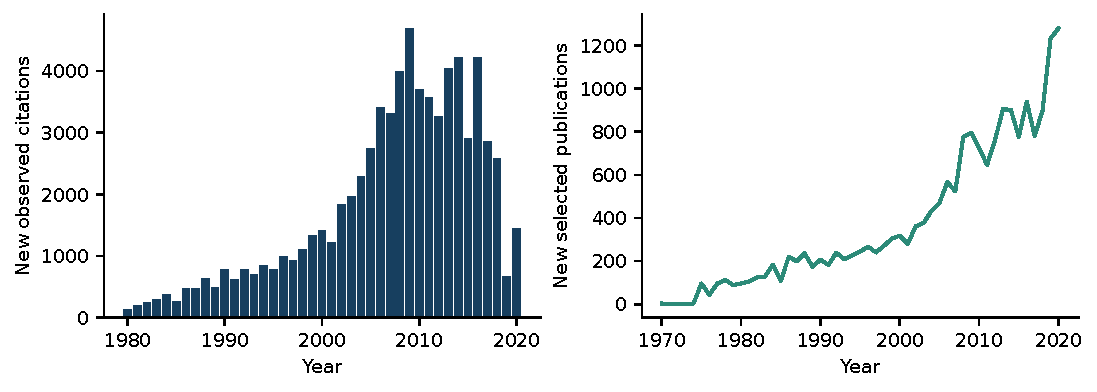
\includegraphics[width=\linewidth]{b_activity.pdf}
\caption{Selected publications and observed within-subgraph citations per year.
The fall in late-period references, despite growing publication counts, cautions
against interpreting the boundary as a change in scientific behaviour.}
\end{figure}

\subsection{M1: annual versus cumulative structure (H1)}
On the common set of 19,150 born nodes in 2020, the annual graph contains 1,450
citations and the cumulative graph 73,269. Mean total degree is respectively
0.151 and 7.652; directed density is $3.95\times10^{-6}$ and
$2.00\times10^{-4}$. The weak largest-component fractions are 0.0523 and 0.6405,
with 17,966 and 6,782 weak components. Cumulative weak clustering is 0.1241.
Annual weak clustering is exactly zero in every year: each retained annual edge
joins a new paper to an older paper, making that snapshot bipartite. This zero is
therefore a consequence of the year convention, not independent evidence for a
social or temporal mechanism.

Over 1-, 2-, 5- and 10-year trailing windows, mean relative ranges are 1.798 for
both density and mean degree, 2.361 for weak clustering, and 1.114 for the
largest-component fraction. Density and degree have identical sensitivity here
because the node denominator is fixed within an endpoint.
\textbf{Verdict on H1:} structural descriptions depend strongly on window choice
in this induced citation graph; some differences are definitional rather than
independent discoveries about temporal correlations.

\begin{figure}[H]
\centering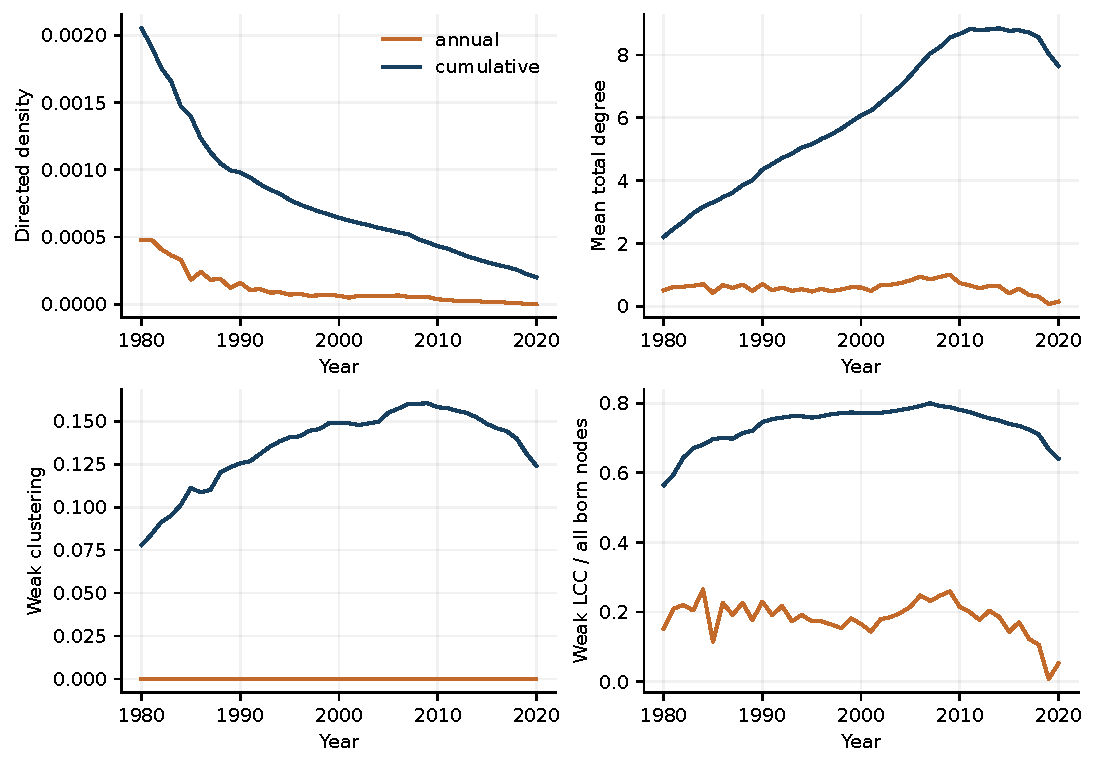
\includegraphics[width=.95\linewidth]{b_aggregation.pdf}
\caption{Measured annual and cumulative graphs with a common born-node denominator.
Clustering and connectivity use the weak projection. Zero annual clustering is
imposed by strict publication-year ordering.}
\end{figure}
\begin{figure}[H]
\centering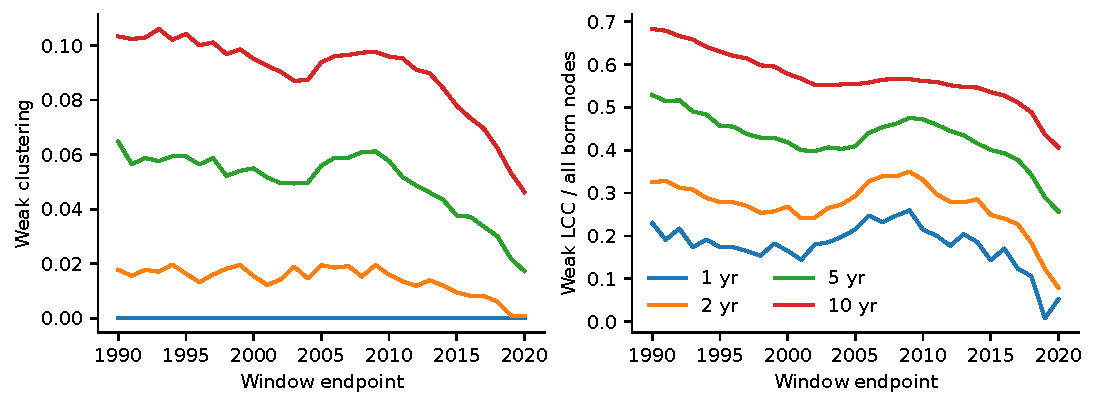
\includegraphics[width=\linewidth]{b_window_sensitivity.pdf}
\caption{Clustering and connectivity under trailing windows. All panels include
already-published isolates; changing the denominator would answer a different question.}
\end{figure}

\subsection{M2c-1: preferential attachment (H4a)}
The conditional degree kernel yields $\alpha=0.7136$, with descriptive
95\% citing-year bootstrap interval $[0.6928,0.7297]$ for
$\Pi(k)\propto(k+1)^\alpha$. Across 20 realizations, P3a gives
$0.00059\pm0.00508$ and the calibrated age-only P3b gives
$-0.65118\pm0.00532$ (mean $\pm$ sample SD). The observed exponent exceeds
every null value; the one-sided empirical probability is $1/21=0.0476$ for
each comparison. This is the coarse minimum resolution of 20 draws, not a
high-precision significance claim or a multiple-testing-adjusted result.

The positive association persists for degree offsets 0.5 and 2
($\alpha=0.6040,0.8576$), the two observation halves (0.6844, 0.7214),
cutoff 2015 (0.7218), and the core SIGMOD/VLDB/ICDE venue-family subset
(0.7309). The numerical exponent depends on the offset.
\textbf{Verdict on H4a:} evidence is consistent with sublinear degree preference
beyond an age-only reference model. Unobserved paper fitness, venue coverage and
other heterogeneity prevent a causal interpretation of $\alpha$.

\begin{figure}[H]
\centering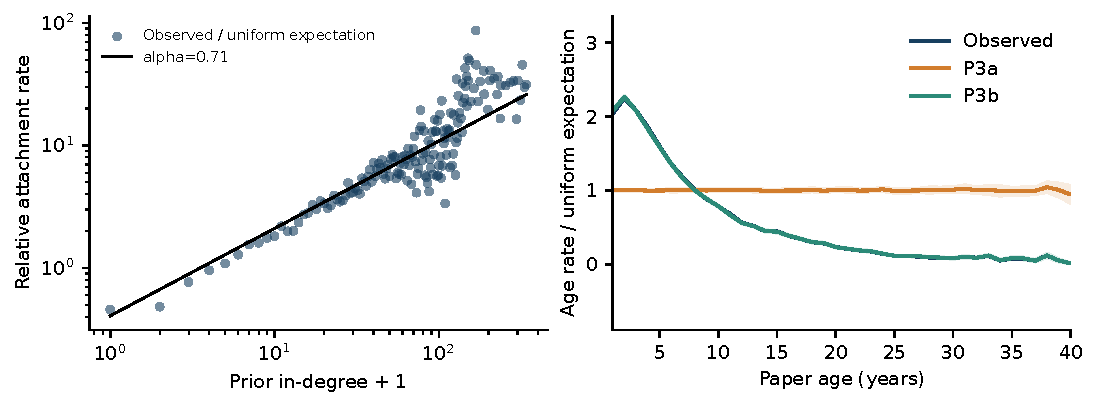
\includegraphics[width=\linewidth]{b_attachment_ageing.pdf}
\caption{Prior-degree attachment and exposure-adjusted ageing. Kernel points with
at least five hits are shown for legibility; the conditional exponent uses all
supported degree classes. The display line uses a pooled normalization, whereas
the estimator conditions on each citing year. Null bands are mean $\pm$ SD.
P3b's ageing agreement is expected from its in-sample calibration.}
\end{figure}

\subsection{M2c-2: ageing and model comparison (H4b)}
Among the declared families, the lognormal target-preference kernel has the
lowest AIC (\autoref{tab:b-age}). Its parameters are
$\mu=1.8584$ and $\sigma=1.1078$, corresponding to the underlying continuous
lognormal scale $\exp(\mu)=6.41$ years. This scale is not the mean age of the
observed citations, because annual target availability also enters the likelihood.
Across all retained events, mean citation age is 5.711 years, versus $11.457\pm0.034$ under P3a and
$5.717\pm0.018$ under P3b. The latter similarity validates the fitted control's
calibration rather than supplying independent evidence for ageing.

\begin{table}[H]
\centering
\begin{tabular}{lrr}
\toprule
Age kernel & Number of parameters & $\Delta\mathrm{AIC}$\\
\midrule
Lognormal & 2 & 0.0\\
Exponential & 1 & 537.8\\
Power-law decay & 1 & 9,360.5\\
Uniform target choice & 0 & 41,796.7\\
\bottomrule
\end{tabular}
\caption{Models compared on the same observations and at-risk age support.
The grid permits ages up to 60; this dataset supplies at most 50 years of exposure.}
\label{tab:b-age}
\end{table}

Lognormal is also preferred within all three target-publication cohorts
(1970--1989, 1990--1999 and 2000--2009), and in both observation halves.
However, fitted cohort parameters differ: for 2000--2009 papers the estimated
$\exp(\mu)$ is about 25.5 years, beyond that cohort's longest available follow-up.
Its unobserved tail must not be interpreted as a measured lifetime.
\textbf{Verdict on H4b:} age-independent target choice is inadequate in these data;
a lognormal age-preference kernel is best among the tested forms. The result is
marginal ageing and does not separately identify obsolescence, fitness or coverage.

\begin{figure}[H]
\centering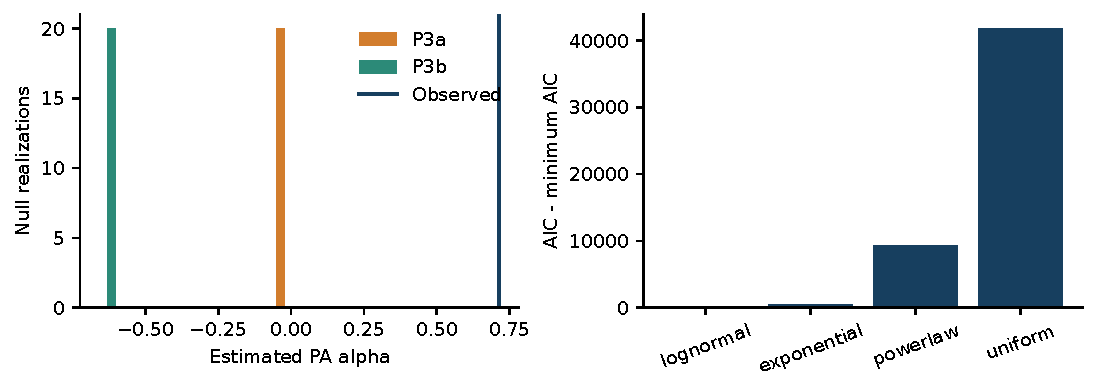
\includegraphics[width=\linewidth]{b_null_and_age_models.pdf}
\caption{Degree exponents under P3a/P3b and relative AIC of age kernels.
These diagnostics condition on the selected corpus and the declared risk sets.}
\end{figure}

\subsection{M2c-3: densification without diameter shrinkage (H4c)}
The cumulative graph follows a descriptive densification relation with
$a=1.3426$, $R^2=0.9913$, and a year-resampling interval $[1.2876,1.4062]$.
Densification means superlinear edge growth relative to nodes, not an increase in
$E/[N(N-1)]$: directed density actually falls while cumulative mean degree rises
from 4.350 in 1990 to 7.652 in 2020. The global exponent masks weaker late growth:
$a=1.4548$ in 1990--2004 and 1.0646 in 2005--2020. It is 1.4270 with cutoff 2015,
1.3242 when the 5,486 same-year references are included, and 1.4099 in the core
venue-family subset ($N=14,235$, $E=47,009$).

The sampled weak-LCC effective diameter is 6 hops in every year from 1990 to 2020.
The largest component grows from 1,657 to 12,266 nodes. Repeating the 1990, 2005
and 2020 estimates with 64 and 256 sources again gives 6 hops. In 2020 the null
estimates are $5.40\pm0.50$ (P3a) and $5.95\pm0.22$ (P3b). P3 leaves
$N(t)$ and $E(t)$ unchanged, so it exactly preserves $a$ and supplies no
significance test for densification.
\textbf{Verdict on H4c:} superlinear cumulative growth is observed, but diameter
shrinkage is not detected at the sampled 90th-percentile resolution. These are
separate empirical propositions.

\begin{figure}[H]
\centering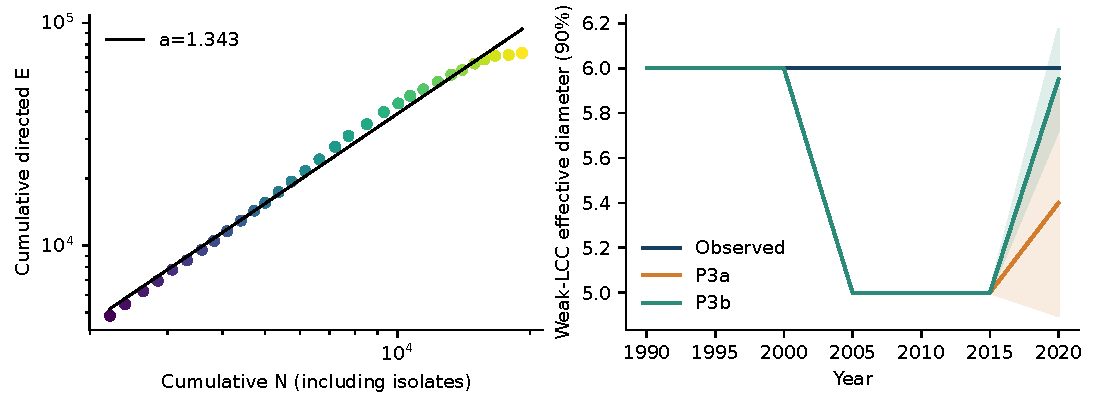
\includegraphics[width=\linewidth]{b_densification_diameter.pdf}
\caption{Densification and sampled weak-LCC diameter. Colour in the left panel
runs from early (dark) to late (yellow) years. Null means and SD are evaluated every
five years. A stable integer-valued 90th percentile does not imply that every
part of the distance distribution is unchanged.}
\end{figure}

\subsection{M2c-4: compact fits versus predictive evidence (H4d)}
The historical reference parameter is fixed at $m=2.00645$. Among 1,019 eligible
papers with at least ten citations by age 15, the prespecified random sample of
500 full histories has median parameters
$(\lambda,\mu,\sigma)=(2.7167,0.8343,1.2375)$.
Their interquartile ranges are respectively $[2.2151,3.4305]$,
$[0.4075,1.3523]$ and $[0.9459,1.7245]$. Median full-history RMSLE is 0.0736,
and median scaled-collapse RMSE is 0.0220 (90th percentile 0.0453).
Full-history boundary fits occur for 10.2\% of papers. These small fitted-sample
errors describe calibration; they do not independently prove a universal curve.

Forecast selection uses only the first five years, yielding 1,220 eligible papers
and a fixed random sample of 500. Every selected fit converges, but 38.6\% hit a
parameter bound, indicating weak identification from short histories. All 500
remain in the primary comparison (\autoref{tab:b-prediction}). The no-ageing PA
baseline can extrapolate explosively; beating it alone is a weak predictive test.

\begin{table}[H]
\centering
\begin{tabular}{llrrr}
\toprule
Target & Model & MAE & Median AE & RMSLE\\
\midrule
Age 15 & WSB & 15.144 & 5.433 & 0.601\\
 & Linear & 17.064 & 13.000 & 0.662\\
 & PA, no ageing & 27,588.0 & 945.937 & 4.601\\
\midrule
Observed 2020 & WSB & 28.016 & 6.786 & 0.778\\
 & Linear & 27.271 & 20.900 & 0.876\\
 & PA, no ageing & $2.79\times10^6$ & 6,466.682 & 7.000\\
\bottomrule
\end{tabular}
\caption{Matched predictions using only ages 1--5 for training, $n=500$ in every
row. The 2020 horizon varies with birth year and remains an observed, censored
within-corpus total, not a lifetime citation count.}
\label{tab:b-prediction}
\end{table}

The paired bootstrap MAE difference (WSB minus linear) is $-1.920$ with 95\%
interval from $-4.471$ to $0.806$ at age 15, and $0.745$ with an interval
from $-4.764$ to $8.128$ at the 2020 endpoint. Both include zero. WSB has smaller RMSLE
and median error, but no clear mean-absolute-error advantage over linear
extrapolation. Restricting to the 307 interior fits improves WSB's age-15 MAE to
9.991, versus 18.547 for linear, but this selected subset cannot replace the
all-paper comparison.
\textbf{Verdict on H4d:} three parameters compactly describe these selected
histories; superiority over a simple linear predictor is not established.

\begin{figure}[H]
\centering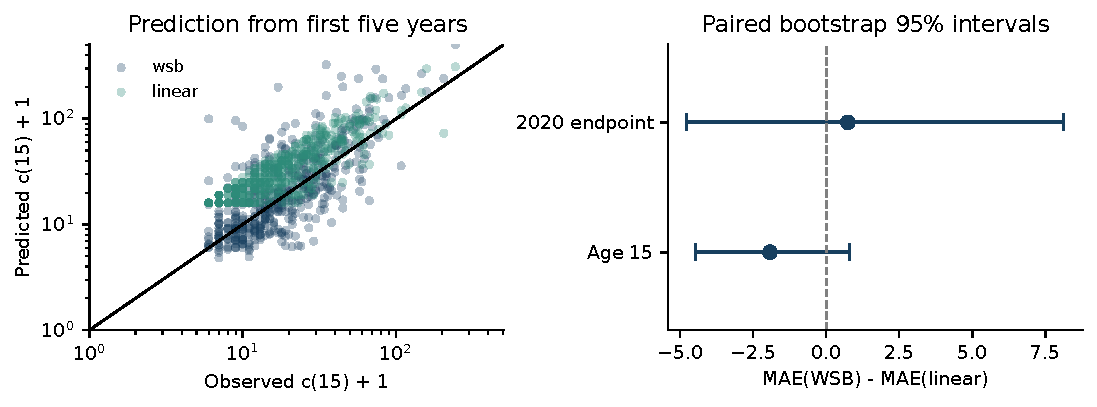
\includegraphics[width=\linewidth]{b_wsb_validation.pdf}
\caption{Held-out prediction and the paired MAE differences versus linear.
Negative differences favour WSB; both 95\% intervals cross zero. The much weaker
no-ageing PA baseline is reported in \autoref{tab:b-prediction} and the full
three-panel diagnostic asset \texttt{b\_wsb.pdf}.}
\end{figure}

\subsection{Reproducibility, robustness and scope}
All five experiment blocks and 40 null graphs completed in serial PBS main job
1500361 on CN-016, with four requested CPU cores, no GPU, exit status 0 and
2\,min\,54\,s wall time including the archive stage. Preparation job 1500299 also
exited 0. Thirteen known-answer unit tests and the formal raw-edge/forecast
selection audit passed. Every null preserves exact source/year counts, distinct
references and strictly older targets. First-ten versus all-twenty mean exponents
are 0.00055 versus 0.00059 for P3a and $-0.65320$ versus $-0.65118$ for P3b.

The exact environment lock, seeds, individual forecasts, fitted parameters,
bootstrap draws, all null edge lists, original-year ties and filtering counts are
saved in the shared summary table (\path{results/b_summary.csv}).
The raw archive SHA-256 is
\begin{center}\small\ttfamily
729cc2c107d8abbe586d9801340246fd94e94d916ba1cebe64dd93a399f0cd28
\end{center}
and matches its persistent HPC-home copy. Conclusions concern one induced
subfield corpus. Missing external citations, venue-name coverage, recorded-year
inconsistencies, annual time resolution, changing late-period reference coverage,
right censoring and fitted-sample selection limit generalisation. No comparison
with PS or CM is inferred before their measured results are available.
